\documentclass[11pt]{article}
\usepackage[margin=1in]{geometry}
\usepackage[T1]{fontenc}
\usepackage{lmodern}
\usepackage{amsmath,amssymb}
\usepackage{booktabs,tabularx,longtable,array}
\usepackage{graphicx}
\usepackage{xcolor}
\usepackage{enumitem}
\usepackage{listings}
\usepackage{float}
\usepackage[hidelinks]{hyperref}
\usepackage{caption}

\definecolor{nabla}{HTML}{1F4E79}
\definecolor{codebg}{HTML}{F5F5F5}
\hypersetup{colorlinks=true,linkcolor=nabla,urlcolor=nabla,citecolor=nabla}
\lstset{basicstyle=\ttfamily\small,backgroundcolor=\color{codebg},frame=single,
  rulecolor=\color{gray!40},breaklines=true,columns=fullflexible,keepspaces=true}
\setlist{itemsep=2pt,topsep=4pt}
\newcolumntype{L}{>{\raggedright\arraybackslash}X}
\newcommand{\code}[1]{\texttt{#1}}
\graphicspath{{../img/}{../img/full/}}

\title{\textbf{\color{nabla}$\nabla$ nabla}\\[4pt]
\large A point-in-time, regime-aware factor book\\
Model specification, results and project record (v1.4)}
\author{Team nabla\\ Ezekiel Galvez (quant: pipeline, backtester, API)\\ Jesse (finance: factors, risk rules, pitch)\\
RowdyHacks Finance Track, UTSA Investment Society --- \textbf{1st place}}
\date{October 2026}

\begin{document}
\sloppy
\maketitle

\begin{abstract}
\noindent nabla is a long-only, weekly-rebalanced, 15-stock US equity book for a \$1M portfolio. Each week it filters the
universe to liquid names, scores them on four published factors (12-1 momentum, guidance velocity, quality and value)
z-scored within groups of stocks that move together, holds the top 15 at roughly equal weight with entry/exit bands,
caps on names, groups, earnings exposure and book beta, and moves 25\% to cash when a rule-based S\&P 500 stress flag is
on. Every input is point-in-time: signals use data through the prior close, fundamentals count from their filing date,
and the model is frozen in configuration files. From January 2018 to the data cutoff (August 2026), net of modeled
trading costs, v1.4 returned \textbf{15.9\% a year} against 13.0\% for the S\&P 500, with Sharpe 0.78 (S\&P 0.73) and
a 33\% maximum drawdown (S\&P 34\%). On six held-back months, opened once, the model (v1.3) returned +19.7\% (S\&P
+11.1\%). This document records the full specification, every test (including those that failed and were not
shipped), the deployment, the known limits, and next steps.
\end{abstract}

\tableofcontents
\newpage

%======================================================================
\section{Summary of what was built}

\begin{table}[H]\centering\small
\begin{tabularx}{\textwidth}{lL}
\toprule
Area & Completed \\
\midrule
Data retrieval & \code{statevector} SDK loaders for prices, opens, state vector, fundamentals, filing calendar,
corporate actions; per-year on-disk cache; split adjustment; point-in-time fundamentals by filing date. \\
Stock grouping & Consensus k-means return clusters (20 seeds $\times$ 3 windows) refit every January on prior data,
frozen in \code{config/clusters.json} (the data has no industry codes). \\
Stock scoring & Liquidity filter; five factors computed (four weighted); winsorize, z-score within cluster, clip;
fixed-weight composite with missing $=0$. \\
Portfolio rules & Top 15 with entry/exit bands, 4 names per group, 10\% per name, 6\% for names reporting within 30
days, 2-point no-trade band, beta cap 1.2 (v1.4), 25\% \code{CASHHOLDING} under stress. \\
Regime & Stress flag (trend + volatility, two-week hysteresis), shipped. Panic rule and a two-state Hidden Markov
model built and tested, both rejected. \\
Costs & Half-spread by liquidity tier plus Amihud price impact; flat 10 bps judges' schedule as an alternative. \\
Backtester & Weekly event loop that calls the same decision function as the live model; close or next-open fills;
metrics, CAPM, rolling windows. \\
Validation & Five-bucket factor test, weekly rank IC with Newey--West $t$, random books, one-day delay, drop-one-factor,
double costs, regime ladder, HMM test, return variants, one-shot holdout, beta cap, stress-test suite with 24
parameter perturbations, crisis windows, Monte Carlo of the judged window. \\
Statistics & Newey--West $t$-stats, paired stationary block bootstrap, deflated Sharpe ratio, pre-registered ship rules. \\
API & FastAPI service: \code{/health}, \code{/portfolio/holdings}, \code{/backtest}, \code{/screen}, \code{/asof}
(rubric, 100/100), \code{/model}, \code{/decide} and \code{/decisions} (judges' replay), offline mode from the
cache, background warm-up. \\
Deployment & Laptop + Cloudflare quick tunnel, later an ngrok static domain; runbook; \code{scripts/practice.py}
mimics the judges' calls. \\
Documentation & \code{docs/AUDIT.md} (every decision), README, HANDOFF, judge Q\&A, pitch deck, charts. \\
Tests & 70 unit and integration tests on a synthetic dataset (\code{pytest}). \\
\bottomrule
\end{tabularx}
\caption{Scope of the project.}
\end{table}

\begin{table}[H]\centering\small
\begin{tabular}{lrrr}
\toprule
Jan 2018 -- Aug 2026, net of costs & nabla v1.4 & S\&P 500 & EW liquid universe \\
\midrule
Return per year & 15.9\% & 13.0\% & 12.1\% \\
Volatility per year & 21.9\% & -- & -- \\
Sharpe ratio & 0.78 & 0.73 & 0.64 \\
Max drawdown & 33.2\% & 33.9\% & 38.9\% \\
Beta, alpha vs S\&P ($t$) & 0.97, +3.5\% (0.89) & -- & -- \\
Turnover per year & 8.6$\times$ & -- & 4.5$\times$ \\
\bottomrule
\end{tabular}
\caption{Headline results of the shipped model.}
\end{table}

%======================================================================
\section{The challenge}

The RowdyHacks Finance Track (run by the UTSA Investment Society) asked for an AI that makes portfolio decisions for
a \$1M book on the organizers' \code{statevector} dataset: about 1,250 US stocks with daily prices, a daily ``state
vector'' of derived features, options panels, filed fundamentals, a filing calendar and corporate actions. The trailing
30 calendar days were a sealed holdout.

\paragraph{Judging.} Two artifacts: a running endpoint and a public repository.
\begin{itemize}
\item A deterministic 100-point rubric (\code{check.py}) called \code{GET /health}, \code{GET /portfolio/holdings}
(shape, long-only, weights sum to $1\pm0.01$, tickers in the universe), \code{POST /backtest} (metrics must match the
reference engine within 2\%), \code{GET /screen}, \code{GET /asof} (no rows dated after the request), all within a 30 s
timeout.
\item A decision-series rubric added on the last day: \code{POST /decisions} with a window returns a chronological series
of target portfolios (integer \code{decision\_id}, \code{information\_cutoff} $\le$ \code{decision\_time} $<$
\code{execution\_time}, max 20\% per name, weights sum to 1), which the judges replay through their own data.
\item A repository audit: it runs, the finance logic is original, it respects point-in-time data, it uses the dataset.
\end{itemize}
Scoring was mostly on total return, with Sharpe and drawdown also counted. Cash is held as the \code{CASHHOLDING}
pseudo-ticker (0\% return, no fees). Trading costs are 10 bps per dollar traded in the reference engine.

\paragraph{Design consequence.} The judged window is about 21 trading days, which is mostly noise for any model. We
therefore favored a few robust, documented signals and explicit risk limits over complex models, and made every
decision a deterministic function of data available at its cutoff.

%======================================================================
\section{System architecture}

\begin{table}[H]\centering\small
\begin{tabularx}{\textwidth}{lL}
\toprule
Module & Role \\
\midrule
\code{src/nabla/data.py} & SDK access, trading calendar, per-year cache, split adjustment, fundamentals and state-vector loaders, S\&P series. \\
\code{src/nabla/fundamentals.py} & Point-in-time fundamentals: filing match, TTM sums, quality and value definitions, SUE/PEAD. \\
\code{src/nabla/clusters.py} & Consensus return clusters, yearly schedule, adjusted Rand index. \\
\code{src/nabla/pipeline.py} & Loads all inputs for a window (prices, groups, fundamentals, splits). \\
\code{src/nabla/factors.py} & Price features, factor table for one date, liquidity filter. \\
\code{src/nabla/combine.py} & Winsorize, z-score within group, clip, fixed-weight composite. \\
\code{src/nabla/book.py} & Selection with bands and group cap, capped equal weights, beta limit, no-trade band, cash line. \\
\code{src/nabla/regime.py}, \code{markov.py} & Stress and panic flags with hysteresis; two-state Gaussian HMM (not shipped). \\
\code{src/nabla/costs.py} & Spread and impact cost model, ADV cap. \\
\code{src/nabla/model.py} & The weekly decision: filter $\to$ composite $\to$ book $\to$ beta cap $\to$ cash. \\
\code{src/nabla/sim.py} & Backtest loop, metrics. \\
\code{src/nabla/live.py}, \code{decide.py} & Live book with state rebuild; replay records, decision series, offline series. \\
\code{src/nabla/stats.py} & Newey--West, block bootstrap, deflated Sharpe, rank IC. \\
\code{app/main.py} & FastAPI service. \\
\code{scripts/} & \code{run\_backtest}, \code{audit}, \code{stress}, \code{build\_book}, \code{build\_series}, \code{fit\_clusters}, \code{fit\_markov}, \code{practice}. \\
\code{config/} & \code{model.json} (all settings), \code{clusters.json}, \code{book.json}, \code{markov.json}. \\
\bottomrule
\end{tabularx}
\caption{Repository layout (\url{https://github.com/envezdezeke/nabla}).}
\end{table}

\noindent One weekly decision flows as:
\begin{center}
data through $t-1$ $\to$ liquidity filter $\to$ factor table $\to$ z-scores by cluster $\to$ composite\\
$\to$ bands and caps $\to$ beta cap $\to$ stress cash $\to$ target weights (sum to 1).
\end{center}
The backtest, the live book and the replay endpoints all call the same \code{model.decide}, so backtest $=$ replay.

%======================================================================
\section{Data retrieval}

\subsection{Access and caching}
The \code{statevector} SDK reads parquet panels from the organizers' server (\code{SV\_DATA\_ROOT} plus a per-team
bearer token \code{SV\_DATA\_TOKEN}, never committed). The hosted server stores one file per trading day, so a
multi-year backtest is thousands of requests. \code{data.\_cached\_years} fetches each panel one calendar year at a
time and keeps it in \code{artifacts/cache}; a year is refetched only if the request runs more than a long weekend past
its last cached day. (An early bug never refreshed a cached year, which froze the live book at February 2026; it was
fixed with a test.) The trading calendar comes from the server manifest; weekdays inside the data with no prints are
treated as holidays (this fixed a Labor Day execution date).

\subsection{Prices and corporate actions}
Daily close and volume are pivoted to date $\times$ ticker frames. Splits come from \code{corporate\_actions}
(\code{kind = split}); a back-adjustment is applied only where the raw price jump at the ex-date actually exists, since
some histories are already adjusted. Opens are adjusted with the same factors for next-open fill tests.
\code{/backtest} later adopted the judges' own \code{apply\_split\_factors} after the organizers updated their
reference (AAPL's 4:1 split in the 2020 rubric window).

\subsection{Fundamentals, point in time}
\code{fundamentals\_actuals} column names were undocumented, so each field is resolved from a candidate list (EPS,
sales, EBIT, EBITDA, net income, free cash flow, net debt, gross margin; no total assets or equity exist).
\code{explore/04\_fundamentals\_check.py} confirmed flows are quarterly (summing four quarters gives TTM) and EPS is
already restated for later splits (AAPL 2019 EPS 0.55 = reported \$2.18/4).

Each quarterly row becomes knowable at its filing: matched to the report calendar's first filing for that
\code{period\_end} within 120 days, usable from the day after the filing date (or the acceptance timestamp when
present). Unmatched rows use a conservative 60-day lag after period end (34\% of 2018 rows, 2\% of 2026 rows).
TTM requires four quarters within about nine months.

\subsection{State vector and benchmarks}
From the daily state vector we use \code{guidance\_range\_velocity}, \code{atm\_iv}, \code{log\_fv\_gap} and
\code{days\_to\_next\_report}. The S\&P 500 index series drives the regime flags, betas and benchmarks. The universe
has almost no financials and no SPY.

\subsection{Stock groups: consensus clusters}
With no industry codes in the data, groups are built from co-movement. On each January 1, using only earlier prices:
\begin{enumerate}
\item For each window $w\in\{252,504,756\}$ days, standardize returns, take loadings on the top 10 principal
components (unit-normalized), and run k-means ($k=10$, k-means++ start) with 20 seeds.
\item Co-assignment matrix $S_{ij} = \#\{\text{runs with } i,j \text{ together}\}/\#\{\text{runs with both}\}$.
\item Average-linkage hierarchical clustering on $1-S$, cut finer until 10 groups of at least 15 names exist; small groups fold into the big group they co-cluster with most.
\item Names with at least 60 days of history join the group whose average return they correlate with most.
\end{enumerate}
Year-to-year agreement (adjusted Rand index) roughly doubled versus a single k-means fit (about 0.45 vs 0.23). The old
single fit had produced a lucky 17.6\% a year; the stable method gives 14.2\% on the same period, and the 17.6\% figure
was withdrawn.

%======================================================================
\section{Stock scoring}

\subsection{Liquidity filter}
A name is eligible on date $t$ if its 20-day average dollar volume is at least \$50M, its price is above \$5, it has a
year of prices, and it is not in the least liquid 10\% of the survivors by Amihud illiquidity
\[
\text{ILLIQ}_i = \frac{10^6}{21}\sum_{d=t-20}^{t} \frac{|r_{i,d}|}{P_{i,d}V_{i,d}}.
\]
About 460 names pass on a typical date.

\subsection{Factors}
All are computed on data through the prior close.
\begin{itemize}
\item \textbf{Momentum 12-1:} $P_{t-21}/P_{t-252}-1$ on split-adjusted closes (Jegadeesh--Titman), skipping the
reversal-prone last month.
\item \textbf{Guidance velocity:} the state vector's \code{guidance\_range\_velocity}: how fast company guidance is
being revised; investors under-react, so prices drift.
\item \textbf{Quality:} the data lacks assets and equity, so quality is a percentile blend (each component ranked,
centered at 0) of gross margin, operating margin (EBIT/sales), FCF margin and low leverage ($-$net debt/EBITDA),
requiring at least two components. Rank blending stops tiny-sales names with margins of $\pm20$ from dominating.
\item \textbf{Value:} TTM EPS / price (earnings yield); loss-makers set to 0 so they rank last together.
\item \textbf{Volatility premium (weight 0 since v1.1):} $-\log(\text{IV}_{30}/\text{RV}_{21})$.
\item \textbf{Built for tests, weight 0:} PEAD (standardized unexpected earnings, Section~\ref{sec:variants}) and
252-day beta vs the S\&P 500, $\beta^{s} = 0.67\beta + 0.33$.
\end{itemize}

\subsection{Composite}
Each factor is winsorized at the 1st/99th percentile, z-scored within its cluster (whole cross-section if the group has
fewer than 5 names), and clipped at $\pm3$. With fixed weights $w_f$ and missing values set to 0,
\[
s_i = \frac{\sum_f w_f\, z_{i,f}}{\sum_f w_f},
\]
dividing by the fixed total rather than each stock's available weight, so names with fewer factors are not favored.
Shipped weights: momentum 1, guidance velocity 1, quality 1, value 1, volatility premium 0.

%======================================================================
\section{Portfolio construction}

\begin{table}[H]\centering\small
\begin{tabularx}{\textwidth}{lL}
\toprule
Rule & Specification \\
\midrule
Book size & 15 names. \\
Entry / exit bands & A new name enters only from the top 15; a held name stays while ranked $\le 30$. \\
Group cap & At most $\lfloor 0.30 \times 15\rfloor = 4$ names per cluster; unclustered names are capped too. \\
Weights & Equal weight, then names with a projected report within 30 days capped at 6\% and the excess
redistributed (all names $\le 10\%$). \\
Beta cap (v1.4) & If $\sum_i w_i \beta^{s}_i \cdot (1-\text{cash}) > 1.2$, swap the highest-beta holding for the
best-scored name ranked $\le 30$ with $\beta^{s} < 1.2$ (respecting the group cap); repeat until under the cap or no
candidate remains. Missing beta counts as 1. \\
No-trade band & Weight changes under 2 points are skipped. \\
Stress cash & Under the stress flag, stock weights scale to 75\%; 25\% is \code{CASHHOLDING}. \\
\bottomrule
\end{tabularx}
\caption{Book rules (\code{config/model.json}, \code{book} and \code{regime}).}
\end{table}

\noindent Every record's weights, including cash, sum to 1.

%======================================================================
\section{Regime rules}

\subsection{Stress flag (shipped)}
Weekly, from the S\&P 500 only:
\[
\text{stress}_t = \mathbb{1}\{P_t < \text{MA}_{200}(P)_t\}\;\wedge\;\mathbb{1}\{\sigma_{21,t} > Q_{0.8}(\sigma_{21,\le t})\},
\]
with the 80th percentile on expanding history. The flag turns off only after two straight weeks of false conditions.
It was on in 18\% of weeks (16 in 2020, 44 in 2022). Funding stress from the plan was left out so backtest and live
use identical inputs.

\subsection{Panic rule (built, rejected)}
$\text{panic}_t = \mathbb{1}\{R^{12m}_t<0\}\wedge\mathbb{1}\{\sigma_{21,t}>Q_{0.8}\}$ halves the momentum weight
(Daniel--Moskowitz momentum crashes). It cost about 3\% a year without reducing drawdown.

\subsection{Hidden Markov stress signal (built, rejected)}
A two-state Gaussian HMM on daily S\&P returns (in percent): states calm/stress with means $\mu_k$, volatilities
$\sigma_k$, transition matrix $A$. Parameters are fit by Baum--Welch with a persistence prior (pseudo-counts 200 on the
diagonal, 2 off it, expected stay about 100 days) and deterministic starts. Walk-forward: year $Y$ uses parameters
fit on returns before January 1 of $Y$. Only the forward-filtered probability
\[
\alpha_t(k) \propto \Big(\sum_j \alpha_{t-1}(j)A_{jk}\Big)\,\phi(r_t;\mu_k,\sigma_k)
\]
is used (never smoothed probabilities, which look ahead). Variants: \code{hmm} ($P(\text{stress})$ on at 0.8, off at
0.5 after two weeks), \code{hmm\_trend} (also requires the S\&P below its 50-day average), \code{rule\_or\_hmm}. A ship
rule was written before running. The HMM caught episodes earlier (2022 by three weeks, August 2024 which the rule
missed) but held cash in about 40\% of weeks; \code{hmm\_trend} returned 11.0\% vs 14.2\% (limit: 1 point) and was
rejected. A statistical jump model with a switching penalty is the documented next candidate.

%======================================================================
\section{Trading costs}
For a weight change $\Delta w_i$ on a book of value $B$:
\[
\text{cost} = \sum_i |\Delta w_i|\left(h_i + k\cdot \text{ILLIQ}_i \cdot |\Delta w_i|\, \frac{B}{10^6}\right),
\]
with half-spread $h_i\in\{5,10,20\}$ bps by 20-day dollar-volume tercile among liquid names (20 bps outside the filter)
and $k=1$; missing Amihud counts as the worst observed. Impact therefore grows with the square of trade size. Positions
are limited to 1\% of 20-day dollar volume. The judges' flat 10 bps schedule is available as \code{cost\_model = flat}.
Costs ran about 0.9\% a year at 8$\times$ turnover.

%======================================================================
\section{Backtesting engine}
\code{sim.run} is a daily loop matching the judges' engine: close-to-close returns, missing prints earn 0, weights drift
between rebalances, and a rebalance resets weights at that day's close and pays costs that day. A rebalance on day $t$
uses data through $t-1$ (\code{signal\_lag} $=1$; 2 is the one-day-delay leak test). Options: next-open fills
(old book earns close$\to$open, new book open$\to$close), rebalance on the $k$-th weekday or every $n$ weeks, and a
market series for per-name beta. The book is liquidated at the end. Rebalances are weekly (first trading day of each
ISO week; the live replay decides on the last trading day of the week and executes at the next open).

\noindent Metrics: total and annual return, volatility, Sharpe, max drawdown, turnover, cost paid, rolling 21-day
median/5th/95th/worst, CAPM beta and alpha with $t$-stat, calendar periods.

%======================================================================
\section{Validation and results}

\subsection{Factor evidence}
Five-bucket test (96 month-ends, about 460 names, next 21 days): no factor had $|t|>1.5$; momentum and guidance pointed
the right way, quality, value and the volatility premium the wrong way on this sample (survivorship likely tilts
quality and value backwards). The weekly rank IC over all liquid names (424 weeks, Newey--West $t$) has far more power:

\begin{table}[H]\centering\small
\begin{tabular}{lrr}
\toprule
Factor & Mean IC & NW $t$ \\
\midrule
Momentum & +0.013 & 1.88 \\
Guidance velocity & +0.011 & 2.22 \\
Quality & +0.008 & 1.57 \\
Value & $-0.003$ & $-0.69$ \\
Volatility premium & $-0.008$ & $-2.43$ \\
PEAD & +0.009 & 2.28 \\
Beta & 0.000 & $-0.01$ \\
Composite & +0.009 & 1.91 \\
\bottomrule
\end{tabular}
\caption{Weekly cross-sectional rank IC, 2018 -- Feb 2026.}
\end{table}

\subsection{Development backtest (v1.3, Jan 2018 -- Feb 2026)}
\begin{table}[H]\centering\small
\begin{tabular}{lrrr}
\toprule
& nabla v1.3 & EW liquid & S\&P 500 \\
\midrule
Return per year & 14.2\% & 11.5\% & 12.4\% \\
Total return & +193\% & +142\% & +158\% \\
Sharpe & 0.70 & 0.61 & 0.70 \\
Max drawdown & 33.3\% & 38.9\% & 33.9\% \\
Bad month (5th pct, 21 d) & $-8.2\%$ & $-8.0\%$ & $-7.2\%$ \\
2018 Q4 & $-12.7\%$ & $-15.2\%$ & $-14.0\%$ \\
2020 & +5.4\% & +27.1\% & +16.3\% \\
2022 & $-18.2\%$ & $-19.5\%$ & $-19.4\%$ \\
Turnover per year & 8.4$\times$ & 4.5$\times$ & -- \\
\bottomrule
\end{tabular}
\end{table}

\begin{figure}[H]\centering
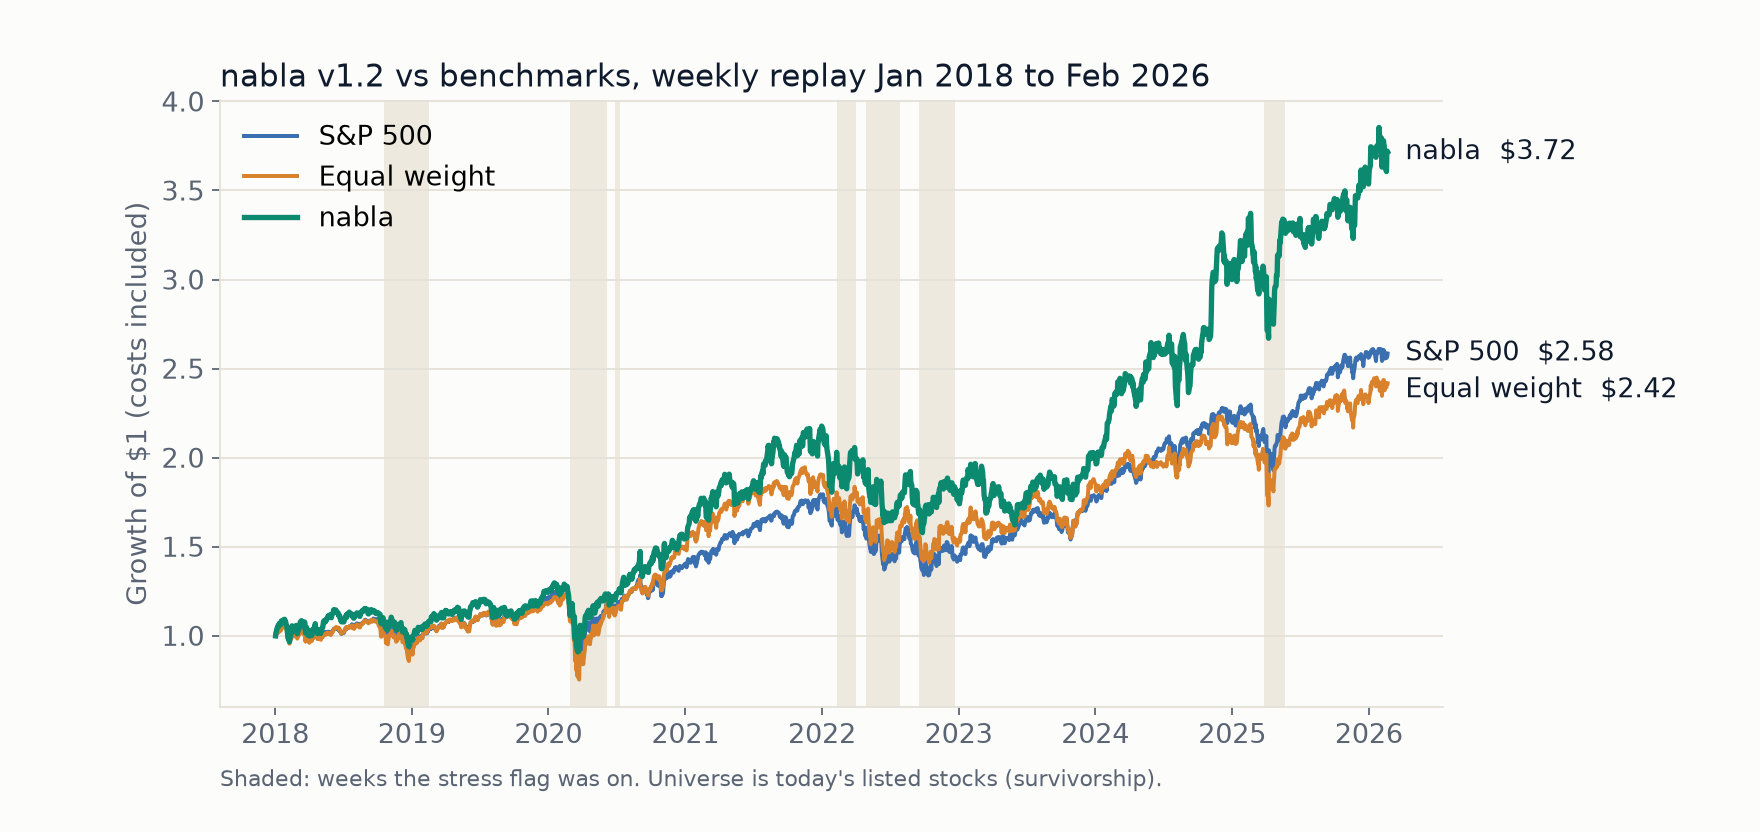
\includegraphics[width=0.85\textwidth]{growth.png}
\caption{Growth of \$1, development period (v1.3).}
\end{figure}

\begin{table}[H]\centering\small
\begin{tabularx}{\textwidth}{lL}
\toprule
Robustness test & Result \\
\midrule
Beta, alpha & 0.98, +2.5\% a year ($t=0.60$): not significant. \\
20 random books (same rules) & Median 10.1\% (4.1\% -- 15.1\%); the model beats 16 of 20. \\
One-day signal delay & 12.4\%: falls, never rises (no look-ahead sign). \\
Next-open fills & 13.2\%, about a point below close fills. \\
Double costs & 13.1\%. \\
Calendar years & Beats equal weight 7 of 9, S\&P 6 of 9 (2024: +47.5\% carried much of the edge). \\
Start years 2018--2022 & Ahead of both benchmarks from every start. \\
Cash rule on/off & Max drawdown 33.3\% vs 40.1\%. \\
Drop one factor & Without momentum 10.4\%, without value 11.3\%; without quality 15.0\%, without guidance 15.4\% (not retuned). \\
\bottomrule
\end{tabularx}
\end{table}

\subsection{Decision log (every change, with its pre-written rule)}
\begin{table}[H]\centering\small
\begin{tabularx}{\textwidth}{lLc}
\toprule
Change & Result & Shipped \\
\midrule
Drop volatility premium (v1.1) & 13.7\% $\to$ 19.2\%, turnover 21$\times$ $\to$ 7$\times$ (old groups) & Yes \\
Panic rule & $-3\%$ a year, no drawdown help & No \\
25\% stress cash (v1.2) & Drawdown 40\% $\to$ 33\% at similar Sharpe & Yes \\
Stable yearly clusters (v1.3) & Withdrew a lucky 17.6\%; honest 14.2\% & Yes \\
HMM stress signal & 11.0\%, failed return limit & No \\
Beta tilt (weight 0.5) & +4.2 pts but beta IC $=0$: market exposure, not skill & No \\
Momentum weight 2 & +2.8 pts, drawdown limit failed & No \\
No cash dial & Same return, +7 pts drawdown & No \\
PEAD factor & +3.5 pts in sample, IC $t$ 2.28; failed one-shot holdout ($-4.4$ pts, beta 1.52) & No \\
Beta cap 1.2 (v1.4) & 14.9\% $\to$ 15.9\%, lower vol and drawdown, final book beta 1.65 $\to$ 1.12 & Yes \\
Mean-variance optimizer & Not built in time (cut rule: ship the simpler rung) & No \\
\bottomrule
\end{tabularx}
\end{table}

\subsection{Return variants and pre-registration}\label{sec:variants}
Before any real-data run we wrote the rule: ship a variant only if annual return is at least 1 point higher, max
drawdown is no more than 5 points worse, and (for factor variants) the factor's weekly IC is positive with NW $t\ge2$.
The winner then faces the six held-back months once and goes live unless it trails by more than 3 points.

PEAD used standardized unexpected earnings
\[
\text{SUE}_{i,q} = \frac{\text{EPS}_{i,q}-\text{EPS}_{i,q-4}}{\operatorname{sd}\big(\text{EPS}_{i,q-k}-\text{EPS}_{i,q-k-4}\big)_{k=1..8}},
\]
live for 91 days after the filing is knowable. It was the only variant to pass in sample and failed the holdout
($+15.3\%$ vs $+19.7\%$; book beta 1.52). It was not retuned, because the holdout was then spent.

\subsection{Held-back six months (opened once)}
\begin{table}[H]\centering\small
\begin{tabular}{lrrrr}
\toprule
Feb 23 -- Aug 21 2026 & Total return & Sharpe & Max drawdown & Beta \\
\midrule
nabla v1.3 & +19.7\% & 1.83 & 7.8\% & 1.13 \\
v1.3 + PEAD & +15.3\% & 1.17 & 15.6\% & 1.52 \\
S\&P 500 & +11.1\% & -- & -- & -- \\
EW liquid & +10.2\% & -- & -- & -- \\
\bottomrule
\end{tabular}
\end{table}

\subsection{Beta cap (v1.4)}
The stress suite found the book entering the judged window at beta 1.65 with 26\% in one memory/semiconductor
cluster. The plan's band upper edge (1.2) was pre-registered as a risk rule (return within 1 point, lower drawdown or
volatility):

\begin{table}[H]\centering\small
\begin{tabular}{lrr}
\toprule
Jan 2018 -- Aug 2026 & v1.3 & v1.4 \\
\midrule
Return per year & 14.9\% & 15.9\% \\
Volatility & 22.6\% & 21.9\% \\
Sharpe & 0.73 & 0.78 \\
Max drawdown & 33.9\% & 33.2\% \\
2025 tariff crash & $-22.9\%$ & $-19.3\%$ \\
Tariff rebound & +20.2\% & +18.5\% \\
Final book beta & 1.65 & 1.12 \\
\bottomrule
\end{tabular}
\end{table}

\subsection{Stress tests}
\code{scripts/stress.py} (factor tables cached across runs) covers:
\begin{itemize}
\item \textbf{Crisis windows:} the model falls slightly less in sell-offs (2018 Q4 $-19.0$ vs $-19.8\%$, Covid crash
$-32.3$ vs $-33.9\%$) and lags rebounds (Covid rebound +38.4 vs +44.5\%, 2022--23 recovery +20.3 vs +28.3\%).
\item \textbf{Regimes:} up-month capture 0.99, down-month 0.84; the edge comes from normal and high-volatility days.
\item \textbf{Judged-window odds} (21 days): $P(\text{loss})=40\%$, $P(\text{beat S\&P})\approx 49$--$52\%$,
$P(\text{loss}>5\%)=14.5\%$; gap vs S\&P from $-4.8\%$ to $+5.9\%$ (5th--95th).
\item \textbf{Parameter perturbations:} 22 of 24 one-at-a-time changes (book size, bands, cash level, group cap,
liquidity floor, 10 random factor-weight draws) beat the S\&P (12.4\% -- 18.7\%); none was adopted.
\item Also: rebalance day and frequency, 3$\times$/5$\times$ costs and the judges' flat fee, next-open fills, Gaussian
noise in the score, random 70\% universes, removing the top winners, today's book replayed through past crises.
\end{itemize}

\subsection{Statistical methods for skill vs luck}
\begin{itemize}
\item Newey--West HAC $t$-stats with Bartlett weights, lag $\lfloor 4(n/100)^{2/9}\rfloor$.
\item Paired stationary block bootstrap (mean block 21 days) of the daily return gap vs the base model.
\item Deflated Sharpe ratio (Bailey--L\'opez de Prado) for the number of variants tried.
\item Power argument: tracking error between variants is about 5--6\% a year, so over 7.5 years the standard error of
an annual-return gap is about 2 points. A 1--2 point improvement cannot reach $t=2$ at the book level; factors must prove
themselves on the full cross-section.
\end{itemize}

%======================================================================
\section{Deployment and API}

\begin{table}[H]\centering\small
\begin{tabularx}{\textwidth}{lL}
\toprule
Endpoint & Behavior \\
\midrule
\code{GET /health} & Model version, data status, warm-up status. \\
\code{GET /portfolio/holdings} & Frozen weekly book (\code{config/book.json}), rebuilt when new data or a new model version appears. \\
\code{POST /backtest} & Reference engine (\code{statevector.run\_backtest}) on split-adjusted cached prices, net of fees. \\
\code{GET /screen}, \code{GET /asof} & Liquidity screen; point-in-time fundamentals (rows dated $\le$ \code{on}). \\
\code{GET /model} & Config, factor coverage, top-30 candidates. \\
\code{GET|POST /decide} & One decision record for an information cutoff (16:00 ET), executed at the next open. \\
\code{POST /decisions} & Weekly series through a window, opening book decided before the window; precomputed in \code{config/series.json} or computed with a time budget. \\
\bottomrule
\end{tabularx}
\end{table}

\noindent Reliability features: stateless state rebuild (each decision replays its own last 8 weeks); weekly books
stored on disk and recomputed in a background loop every 10 minutes; the server index refreshed so new days appear;
a 25 s budget on \code{/decide} with the frozen book as fallback. In \textbf{offline mode} (when the data token was
revoked after submission) the API still starts: \code{/backtest}, \code{/screen} and \code{/asof} read the real cached
data, holdings come from the frozen book, and \code{/decisions} returns the frozen book bought at the window's first
open for windows after its data (and refuses earlier windows rather than look ahead). Hosting was a laptop behind a
Cloudflare quick tunnel (HTTP/2, since venue Wi-Fi blocked QUIC), then an ngrok static domain so the URL survived
restarts. \code{check.py} scored 100/100 on the deployed URL.

%======================================================================
\section{Planned but not implemented}
\begin{itemize}
\item \textbf{Mean-variance optimizer} (cvxpy): $\max_w \mu^\top w - \tfrac{\gamma}{2}w^\top\Sigma w - \sum_i c_i|w_i-w_i^{prev}| - \kappa\|w-w^{EW}\|^2$ with $\mu_i=\beta^s_i m + \lambda\,\text{IC}\,\sigma_{cs}\,s_i$, Ledoit--Wolf covariance, beta band, group and ADV constraints, equal-weight anchor. Cut by the timeline rule.
\item \textbf{Hidden Markov regime model:} built, tested, rejected (Section 6.3); not used in decisions.
\item Lower edge of the beta band (1.10) and the stress preset's 0.90--1.00 band with low-beta swaps.
\item Funding-stress input to the stress flag.
\item Trim rule (trim above 12\% back to 10\%), ``no add the week before earnings'', optional trailing stop, crowding swap.
\item Reinforcement-learning bandit, put-option overlay, partial trading, logistic flag calibration (cut in plan v5).
\end{itemize}

%======================================================================
\section{Known limits}
\begin{itemize}
\item One month is mostly noise; a 15-name book swings 6--8\% in a typical month.
\item Survivorship: the universe is today's listed companies, flattering backtests and likely biasing quality and value.
\item Narrow universe: almost no financials, no SPY.
\item Few stress episodes (2018 Q4, 2020, 2022) behind the cash rule.
\item Skill not statistically proven (alpha $t<1$); choices made on the same sample, mitigated by pre-registration and one holdout.
\item The backtest path depends on where the data window ends (13.7\% vs 14.2\% on the same years); cause not isolated (leading candidate: the \$5 price filter on back-adjusted closes). The replay is unaffected.
\item Costs are modeled, not measured; the edge is thin (one-day delay brings it to S\&P level).
\end{itemize}

%======================================================================
\section{Next steps}

\subsection{Keep the model going}
\begin{enumerate}
\item \textbf{Live out-of-sample tracking:} run \code{decide()} every Friday on new data, log records, and compare to the S\&P and equal weight; after 6--12 months this is the honest test.
\item \textbf{Fix the window-end dependence} by isolating which input changes when data is appended (start with the price filter on adjusted closes).
\item \textbf{Build the optimizer} as rung 4 and judge it on a pre-written rule against v1.4 on new data only.
\item \textbf{Revisit PEAD and a jump-model regime filter} only on data after the cutoff (walk-forward), never on the spent sample.
\item \textbf{Monitor factor IC} monthly with NW $t$; reduce weight on a factor whose IC stays negative for a pre-set period.
\item \textbf{Run 100 random books} for a proper percentile $p$-value.
\item \textbf{Engineering:} cloud hosting (a small VM or container) instead of a laptop; scheduled data refresh; CI running \code{pytest} and \code{check.py}; record the git commit and data hash in \code{model.json}.
\end{enumerate}

\subsection{Other settings}
\begin{itemize}
\item \textbf{Paper and personal trading:} connect the weekly target weights to a broker's paper-trading API (e.g.\ Alpaca or Interactive Brokers) with the same cost model; trade only the no-trade-band-filtered changes.
\item \textbf{Other data:} rebuild the loaders on free/academic sources (CRSP/Compustat through a university, or yfinance plus SEC EDGAR filings with filing dates) and include delisted stocks to remove survivorship bias.
\item \textbf{Other universes:} ETFs (sector and factor rotation with the same regime dial), international equities, or a larger multi-cap universe where long-short decile spreads give statistical power.
\item \textbf{Risk management and compliance:} the stress flag, beta and concentration caps, crisis replays and rolling-window odds generalize to portfolio risk monitoring and limit dashboards (e.g.\ a bank's investment portfolio or a student investment fund).
\item \textbf{Teaching and research:} the pre-registration workflow (rule written, run once, log the result) is a template for actuarial and finance coursework and quant interview projects.
\end{itemize}

%======================================================================
\appendix
\section{Version history}
\begin{table}[H]\centering\small
\begin{tabularx}{\textwidth}{lL}
\toprule
Version & Change \\
\midrule
v1 & Five factors, equal-weight top 15, bands and caps, liquidity filter, cost model, weekly backtest. \\
v1.1 & Volatility premium weight 0 after the drop-one-factor test. \\
v1.2 & 25\% stress cash dial; panic rule rejected. \\
v1.3 & Consensus clusters refit each January, frozen; 17.6\% withdrawn for 14.2\%. \\
v1.4 & Book beta capped at 1.2; shipped and judged; 1st place. \\
\bottomrule
\end{tabularx}
\end{table}

\section{Shipped configuration}
\begin{lstlisting}
version: v1.4
factor_weights: momentum 1, guidance_velocity 1, quality 1, value 1, vol_premium 0
liquidity: min_adv 50e6, min_price 5, amihud_drop_pct 0.90
book: n 15, exit_rank 30, max_name 0.10, sector_cap 0.30, earnings_cap 0.06,
      earnings_days 30, no_trade_band 0.02, beta_max 1.2
regime: method rule, stress_cash 0.25, panic_momentum false
costs: half_spread_bps [5, 10, 20], impact_k 1.0, max_adv_pct 0.01
backtest: start 2018-01-01, holdback_months 6, cost_model plan, book_value 1e6
clusters: k 10, seeds 20, windows [252, 504, 756], n_pc 10, min_size 15
\end{lstlisting}

\section{How to run}
\begin{lstlisting}
pip install -e <starter repo>/sdk -r requirements.txt
export SV_DATA_ROOT=... SV_DATA_TOKEN=...      # never commit the token
python scripts/run_backtest.py                # weekly backtest vs EW and S&P
python scripts/audit.py --only base,random,delay,cost2x,drop,ic
python scripts/stress.py --only windows,book,params
python scripts/build_book.py                  # freeze this week's book
python scripts/build_series.py                # freeze the decision series
uvicorn app.main:app --port 8000
python scripts/practice.py --url http://localhost:8000
pytest -q                                     # synthetic data, no token
\end{lstlisting}

\end{document}
